\documentclass[tikz,border=8pt]{standalone}
\usetikzlibrary{arrows.meta,positioning,decorations.pathreplacing}
\begin{document}
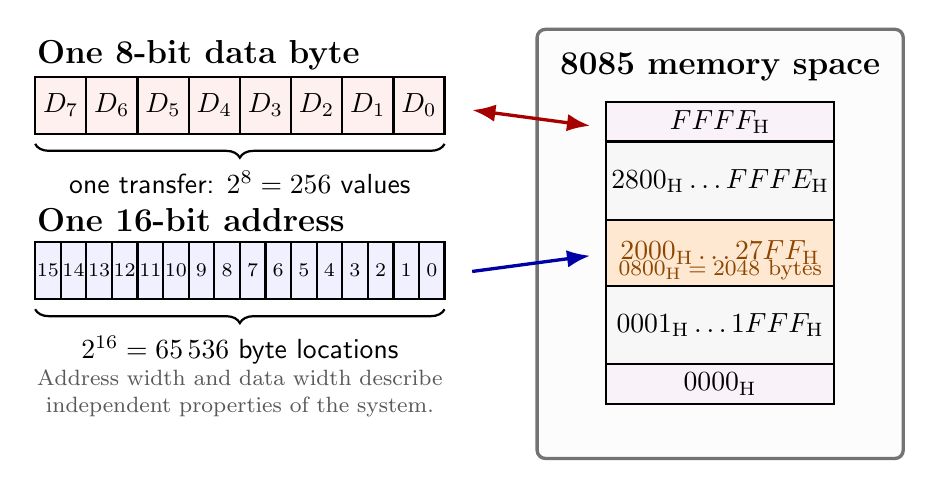
\begin{tikzpicture}[font=\sffamily,>=Latex]
  \node[font=\bfseries\large,anchor=west] at (-.1,2.65) {One 8-bit data byte};
  \foreach \i/\lab in {0/D_7,1/D_6,2/D_5,3/D_4,4/D_3,5/D_2,6/D_1,7/D_0}{
    \draw[thick,fill=red!6] (0.65*\i,1.65) rectangle ++(.65,.72);
    \node at (0.65*\i+.325,2.01) {$\lab$};
  }
  \draw[decorate,decoration={brace,mirror,amplitude=5pt},thick] (0,1.52) -- node[below=6pt]{one transfer: $2^8=256$ values} (5.2,1.52);

  \node[font=\bfseries\large,anchor=west] at (-.1,.55) {One 16-bit address};
  \foreach \i in {0,...,15}{
    \pgfmathtruncatemacro{\bit}{15-\i}
    \draw[thick,fill=blue!6] (0.325*\i,-.45) rectangle ++(.325,.72);
    \node[font=\scriptsize] at (0.325*\i+.1625,-.09) {\bit};
  }
  \draw[decorate,decoration={brace,mirror,amplitude=5pt},thick] (0,-.58) -- node[below=6pt]{$2^{16}=65\,536$ byte locations} (5.2,-.58);

  \node[draw=black!55,rounded corners=3pt,very thick,minimum width=4.65cm,minimum height=5.45cm,fill=black!1] (mapbox) at (8.7,.25) {};
  \node[font=\bfseries\large,anchor=north] at ([yshift=-.2cm]mapbox.north) {8085 memory space};
  \draw[thick,fill=violet!5] (7.25,1.55) rectangle (10.15,2.05);
  \node at (8.7,1.8) {$FFFF_{\mathrm H}$};
  \draw[thick,fill=black!3] (7.25,.55) rectangle (10.15,1.55);
  \node at (8.7,1.05) {$2800_{\mathrm H}\ldots FFFE_{\mathrm H}$};
  \draw[thick,fill=orange!18] (7.25,-.28) rectangle (10.15,.55);
  \node[font=\bfseries,text=orange!55!black] at (8.7,.14) {$2000_{\mathrm H}\ldots27FF_{\mathrm H}$};
  \node[font=\footnotesize,text=orange!55!black] at (8.7,-.08) {$0800_{\mathrm H}=2048$ bytes};
  \draw[thick,fill=black!3] (7.25,-1.28) rectangle (10.15,-.28);
  \node at (8.7,-.78) {$0001_{\mathrm H}\ldots1FFF_{\mathrm H}$};
  \draw[thick,fill=violet!5] (7.25,-1.78) rectangle (10.15,-1.28);
  \node at (8.7,-1.53) {$0000_{\mathrm H}$};

  \draw[->,very thick,blue!65!black] (5.55,-.1) -- (7.05,.1);
  \draw[<->,very thick,red!65!black] (5.55,1.95) -- (7.05,1.75);
  \node[font=\footnotesize,text=black!65,align=center] at (2.6,-1.65) {Address width and data width describe\\independent properties of the system.};
\end{tikzpicture}
\end{document}
